\chapter{Mises à jour de l'expérience}
%\begin{tikzpicture}[remember picture, overlay]
%\node[anchor=north east,inner sep=0pt] at (current page.north east) {
\includegraphics[scale=1]{Fig/Chapter1/g825.png}};
%\end{tikzpicture}


parler des modifications apportées à la manip: cicero, ODT + evap, calibration levitation par oscillations + spin-flip, réparation lévitation...

\section{Mise à jour de l'informatique de l'expérience}
\subsection{Contrôle de l'expérience: passage à la suite Cicero}
\subsection{Développement d'une nouvelle interface d'acquisition et de traitement d'images}

\section{Réparation et recalibration de la lévitation magnétique}
\subsection{Réparation de la lévitation magnétique}
\subsection{Calibration par oscillations}
\subsection{Calibration par radio-fréquences}

\section{Changement du laser telecom et calibration du piège optique}
\subsection{Changement du laser telecom}
\subsection{Calibration du piège optique}
%\subsection{Optimisation de l'évaporation dans le piège dipolaire}

\section{Optimisation de l'évaporation tout-optique}


\begin{comment}

%
%4.1 : Models of confidence in decision-making
%- Signal theory
%- Bayesian theory
%- How to model confidence using attractor network ?
%
%4.2 : How to map data and model
%- Explication
%- Analyse des effets sequentiels dues à la confiance
%- Usefulness of attractor neural networks


%In daily life, the decisions we make are usually accompanied by a feeling of whether the decision was right or wrong. For example, you want to cross the road at a busy intersection. You will need to assess the speed of the vehicles as well as the size of the gaps between the vehicles. To judge if it is safe to cross the road, one should also estimate how trustworthy one’s inferences are about speed and distance. Thus, this ability to estimate the accuracy of a decision is critical in everyday life.
%In this chapter I will first adress different models of confidence in decision-making. In a second part, I will focus on the impact of confidence on sequential effects during perceptual decision-making.

\section{Models of confidence in perceptual decision-making}

%Since the early work on decision-making, confidence judgments have been recorded alongside with decisions. In \cite{peirce1884small}, participants were asked to report their confidence in the perceptual decision they just make. In this work, the task was to discreminate between pressures applied to their fingers and to report their confidence on a four-ratings scale analog to the one describe in the preceeding chapter.  Surprisingly, the confidence ratings of the participants could be described by the following formula:
%\begin{equation}
%	w = c \log \frac{p}{1-p}
%\end{equation}
%with $w$ the degree of confidence, $p$ the probability of being right and $c$ a constant called the index of confidence. However, this type of measure is sensible to many undesirable effects such as the fact that participants interpret differently the confidence scale thus displaying over- or under-confident behavior~\citep{fleming2014measure}. For this reason, current confidence ratings' analysis require more detailed analyses and I will describe the main contempory frameworks of confidence.


\subsection{Signal detection theory (SDT) framework} 
%% TODO: example d'autres seuils ?
%In SDT, the observer receives an observation of evidence $e$~\citep{green1966signal}. This observation is caused by a stimulus and differs depending on the category the stimulus belongs to. However, the evidence $e$ is corrupted by noise, thus the likehoods for the stimulus to belong to one category or the other are overlapping. For example, let us consider two categories $C_1$ and $C_2$ that follow normal distribution with means ($\mu_{C_1}=-0.5$ and $\mu_{C_2}=0.5$) and equal variance ($\sigma_{C_1}^2 = \sigma_{C_2}^2 = 1$) (Figure~\ref{fig:chap4-fig1}.A). The task of the observer is to infer the posterior probability $P(C=C_1 \vert e)$. Using Bayes' rule, this posterior probability can be rewritten as:
%\begin{equation}
%	P(C=C_1 \vert e) = \alpha P(e \vert C_1) \cdot P(C=C_1)
%\end{equation}
%with $\alpha$ a normalization factor computed through the relation $P(e \vert C_1) = P(e \vert C_2) = 1$. In the following I will suppose that $P(C=C_1) = P(C=C_2) = 0.5$ (Figure~\ref{fig:chap4-fig1}.B). 

%\begin{figure}[h!]
%	\centering
%	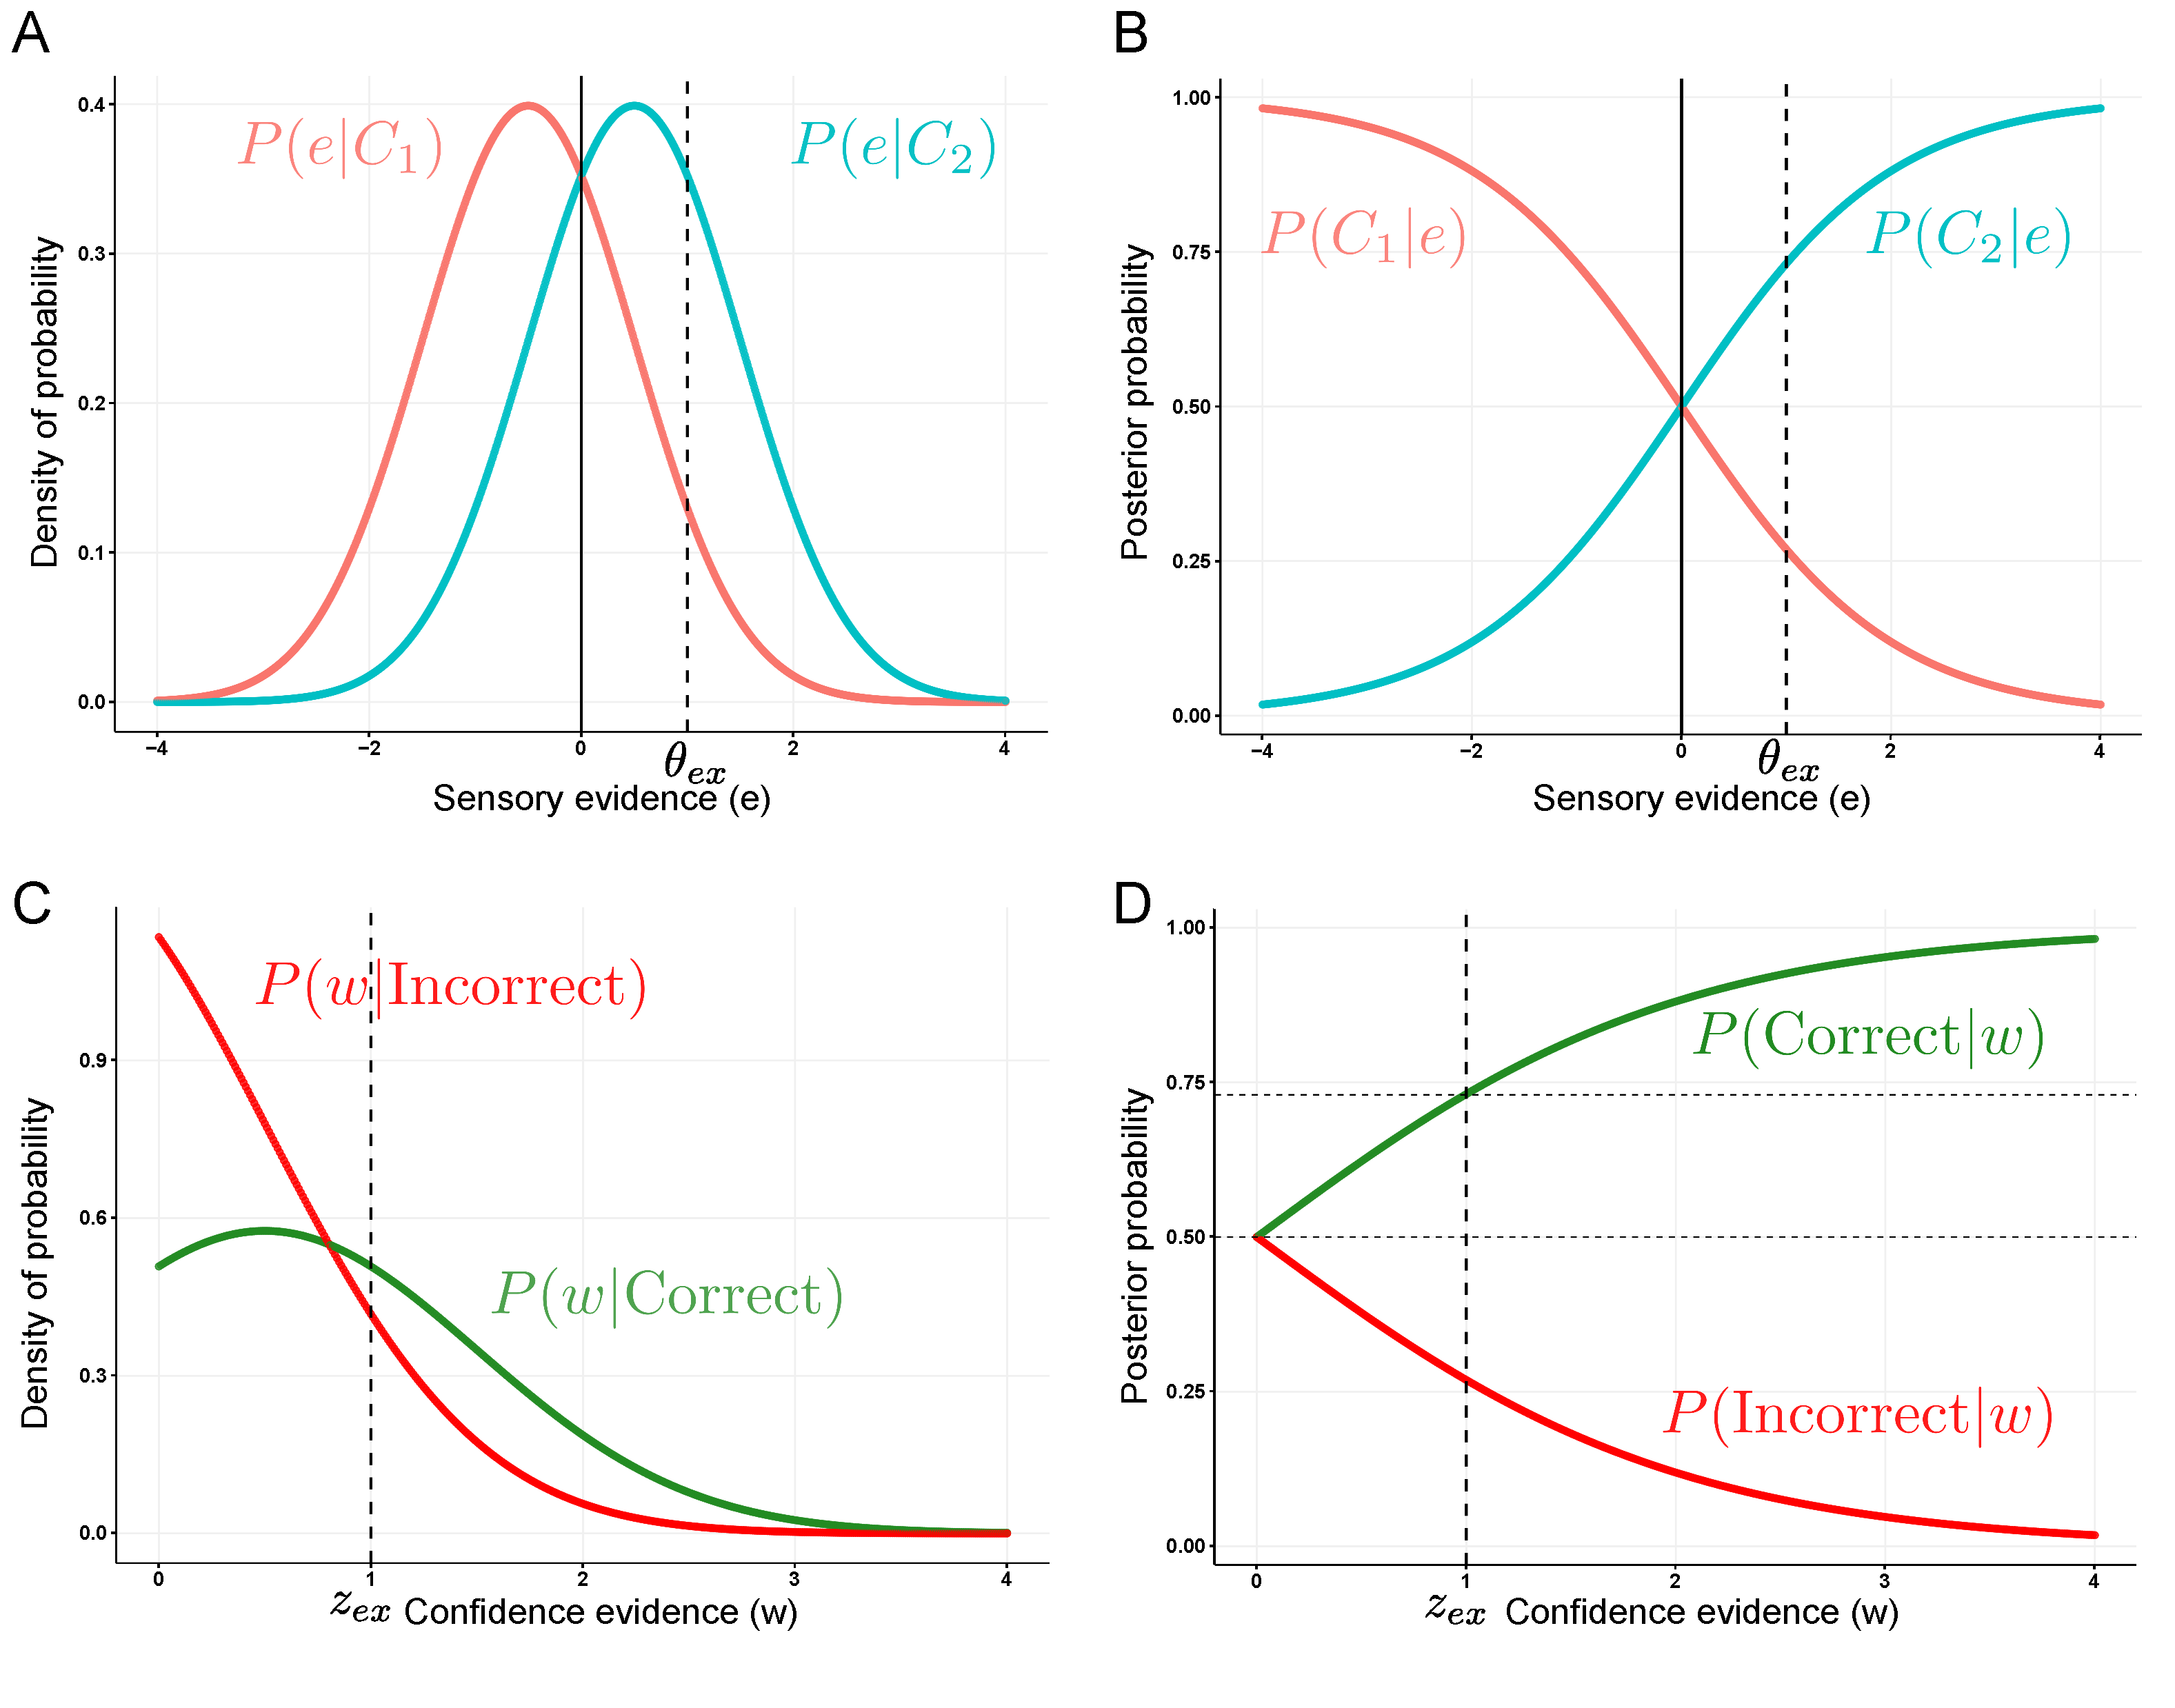
\includegraphics[width=1.0\linewidth]{Fig/Chapter4/fig1.eps}
%	\caption{{\bf Signal detection theory framework.} (A) Density of probability of the two categories $C_1$ and $C_2$ as defines in the text. The line at $0$ denotes the value of the optimal criterion. The dashed line at $\theta_{ex}$ corresponds to a criterion slightly biased towards category $C_1$. (B) Posterior probability of the categories with respect to the sensory evidence $e$. (C) Density of probability of the confidence evidence for correct (green) and incorrect (red) trials. The dashed line at $z_{ex}$ corresponds to an example of a confidence criterion that is slightly underconfident. (D) Posterior probability of the correctness of the trial with respect to the confidence evidence.}
%	\label{fig:chap4-fig1}
%\end{figure}


%To achieve such estimation, the observer places a criterion $\theta$ along the sensory evidence axis (Figure~\ref{fig:chap4-fig1}.A). The chosen category will then be $C_2$ if the sensory evidence $e$ exceeds this criterion, and $C_1$ otherwise. In the setup of Figure~\ref{fig:chap4-fig1}, the symmetry of the problem indicates that the optimal criterion is $\theta = 0$ (Figure~\ref{fig:chap4-fig1}.A), but the observer could choose another value, for example to model biaises in decisions. 	

%The observer's evidence about the correctness of his/her decisions varies along a confidence axis ($w$). There are many possibilities to model the confidence evidence within the signal detection theory framework. For instance, one could assume that the confidence evidence is the distance between the sensory evidence and the criterion $\theta$~\citep{clarke1959two} or that it is the likelihood ratio of the sensory evidence given that the perceptual evidence was correct or incorrect~\citep{galvin2003type}. In the example I am considering, I will assume that the confidence evidence is directly the distance between the sensory evidence and the criterion $\theta$:
%\begin{equation}
%	w = \vert e - \theta \vert
%\end{equation}
%It is important to distinguish between the confidence evidence for correct and incorrect decisions. Indeed, in this analysis of confidence evaluation, the categories "I am correct" and "I am wrong" will play the role of the categories $C_1$ and $C_2$. The likehood of confidence evidence for correct decisions is:
%\begin{equation}
%	P(w \vert \text{Correct}) = P(\vert e - \theta \vert \vert \text{Correct}) = P(e-\theta \vert C_2 ) + P(\theta - e \vert C_1)
%\end{equation}
%This likelihood is illustrated on Figure~\ref{fig:chap4-fig1}.C in the case of an optimal criterion $\theta = 0$. Finally using the Bayes' rule, one can obtain the posterior probability of being correct (or incorrect) with respect to the confidence evidence (Figure~\ref{fig:chap4-fig1}.D).

%%TODO: à finir
%\begin{equation}
%	P(\text{Correct} \vert w ) = k \cdot P( w \vert \text{Correct}) \cdot P(\text{Correct})
%\end{equation}

%\begin{equation}
%P(\text{Incorrect} \vert w ) = k \cdot P( w \vert \text{Incorrect}) \cdot \left(1-%P(\text{Correct})\right)
%\end{equation}
%with $k$ a normalization constant. 

%% TODO: un peu plus d'explications sur les ouvertures et ocmportement du modèle ?

%To decide between high and low confidence trials, the observer places a second criterion $z$ along the confidence evidence axis (Figure~\ref{fig:chap4-fig1}.C). If the evidence $w$ is higher than $z$, the trial is favored towards the high confidence hypothesis. However, it is important to note that, in this case, there is an optimal location for the criterion $z$ too. This location corresponds to the intersection of the likelihood of confidence evidence %(Figure~\ref{fig:chap4-fig1}.C). 
% If the criterion is placed after this value, the observer will show risk-aversion. In contrast if the criterion is placed closer to the origin, it will increases the risk of assigning high confidence to incorrect trials thus being overconfident. To conclude, this framework can show different behaviors observed in the experiments such as risk-aversion and overconfidence. However, SDT models assumes that the decision is made with a fixed amount of time due to the fact that the sensory evidence is drawn from an unique sample. Thus, this model can't describe the relationships between confidence, response time and stimulus difficulty in the case of the two-alternatives forced choice task. %%REFS ?? %% nom de l'expérience ?
 
 
 \subsection{Accumulation of evidence framework}
%ù TODO: cette partie suppose que l'accumulation d'évidence a été discutée dans l'intro.

%To model the dynamics of the decision process as well as the confidence in one's decision, one solution is to use evidence-accumulation models. I focus here on decision model where the decision is made when the accumulation process reaches a specific bound $\theta$. Multiples variations of accumulations can be found in the literature, such as the drift-diffusion model~\citep{ratcliff1978theory,bogacz2006physics} or the independent race model~\citep{raab1962division,vickers1970evidence,merkle2006application}. The IRM being slightly more general than the DDM, I will be using the IRM framework to present the modelisation of confidence, in the case of a two-alternative forced choice task. %% phrase à changer %% description boE

%When an observer $O$ is presented with a stimulus $S$, it initiates two simultaneous races representing the evidence of favor of both options (Figure~\ref{fig:chap4-fig2}.A). In order to model confidence with this model, (Vickers et al.) proposed to define the confidence as the balance of evidence (Figure~\ref{fig:chap4-fig2}.A) at the time of the decision. One should note that this definition means that the losing race plays a role in confidence evaluation, even if it does not play a role in the decision. When the two races are close at the time of the decision, the balance of evidence is small. This means that the confidence is this decision is going to be low, as a small perturbation in the races would have lead to the opposite decision. In contrary, if the races are far apart, the balance of evidence is high and the confidence will be high too. The equations for the IRM are the following:

%\begin{align}
%    \dot x_1 &= \mu_1 + \sigma \eta_1(t) \\
%     \dot x_2 &= \mu_2 + \sigma \eta_2(t) 
%\end{align}
%with $x_1,\, x_2$ the decision variables, $\eta_1, \, \eta_2$ the white noises corresponding to each alternative and $\mu_1,\, \mu_2$ the mean drift of each races.

%I recall that the decision is made once one the races has reached a fixed threshold. This means that the balance of evidence can be characterized only by the state of the losing race at the time of the decision. Without loss of generality, the winning race corresponds to $x_1$, and I define $\Delta x = \theta - x_2$ the balance of evidence at the time of decision. The decision is correct if, indeed, $\mu_1 > \mu_2$. Using Fokker-Planck equation, one can find that: %ùREFS
%\begin{equation}
%    P(\mu_i \, \vert \, x_i ,t ) = \frac{1}{\sqrt{2 \pi \sigma^2/t}} \exp \left(- \frac{\left(\mu_i - x_i/t \right)^2}{2 \sigma^2 t} \right)
%\end{equation}
%The confidence in the decision corresponding to race $1$ is defined by $  P(\mu_1 > \mu_2 \, \vert \, x_2,t,x_1 = \theta)$~\citep{moreno2010decision}. 
%The probability of having chosen the right race corresponds to the probability that a Brownian motion finish at state $\Delta x$ or lower, meaning that the noise was not strong enough to elicit the wrong decision. %% ref equation ?
%This leads to:
%\begin{equation}
%    P(\mu_1 > \mu_2 \, \vert \, x_2,t,x_1 = \theta) = \frac{1}{\sqrt{2\pi}} \int_{- \infty}^{\Delta x /(\sigma \sqrt{t})} \exp \left( -z^2/2 \right) dz %%diff a faire
%    \label{IRM:confidence}
%\end{equation}

%\begin{figure}[h!]
%	\centering
%	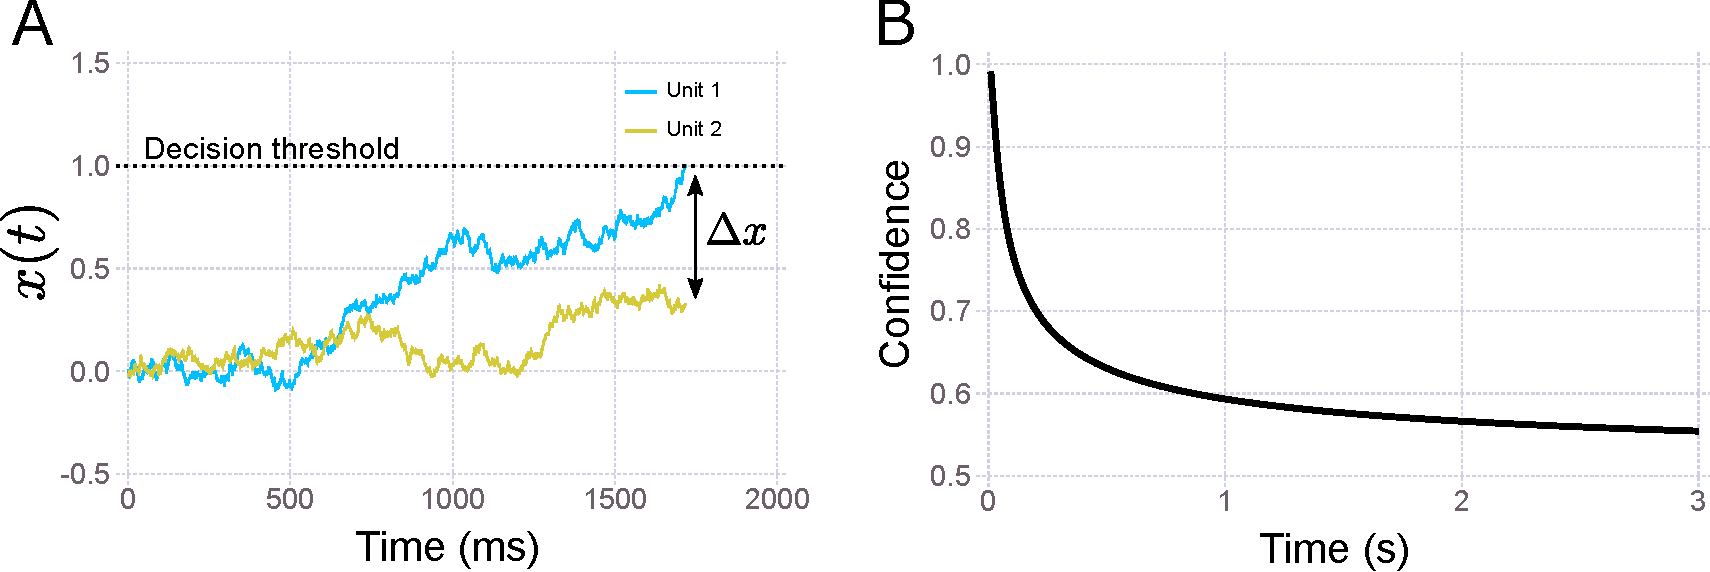
\includegraphics[width=1.0\linewidth]{Fig/Chapter4/IRM.pdf}
%	\caption{{\bf Independent Race Model.} (A): Example of the dynamics for two independent races (denoted by each color). The parameters are $\theta=1$, $\sigma = 1.0$, $\mu_1 = 0.07$ and $\mu_2 = 0.05$. The balance of evidence corresponds to the arrow $\Delta x$ at the time of the decision. (B): Confidence with respect to the decision time (Equation~\ref{IRM:confidence}). The parameters are $\sigma=3$, $\theta=1$ and $x_2=0.5$(the state of the losing race at the time of the decision). }
%	\label{fig:chap4-fig2}
%\end{figure}

%This framework gives a relation between between response times and confidence that is represented in Figure~\ref{fig:chap4-fig2}.B. Confidence is a monotonic function of decision time, that decays from $1$ to $0.5$. This decay is explained by the fact that fast trials are more likely to correspond to higher drift rates, thus higher performances. Experimental measurements have found such decay of confidence with respect to decision times~%\citep{vickers1979decision}. 

%Other models have been proposed to model confidence within an evidence-accumulation framework. Indeed, in the case of DDMs there is no losing race. To use the notion of balance of evidence, it has been proposed that the accumulation process continue after the decision has been reached~\citep{pleskac2010two} 
%and the final location of the process is used as a proxy for confidence. Other models propose to use different DDMs, each of them corresponding to a specific confidence level, the winning DDM determines the confidence level of the trial~\citep{ratcliff2013modeling}. 
%In any cases, all these models have in common the fact that they attempt to characterize decision times, accuracy and confidence, within a perceptual task, using a mechanism based on the balance of evidence.

\subsection{Neural substrates of decision confidence} %% un mot sur modèle biophsique dans le titre ?

%Recent experimental studies have been focused on understanding the representation of confidence, as the subjective probability the decision chosen is correct, within the brain. The first study addressing this question was the one of~\cite{kiani2009representation}. The authors recorded from neurons in the lateral intraparietal cortex (LIP) of behaving monkeys. The animals were performing a specific version of the random dot motion task (RDM) %REFS
%specially designed to study confidence (opt-out task). In addition to the two choices corresponding to the dots moving towards left or right, the monkeys could chose a third target corresponding to a small but certain reward. Interestingly, the monkeys chose the sure option in a way that is correlated with the chance of making the correct decision. %% REFS et figure reproduite ?
%They chose the sure target more frequently when the probability of making the correct decision was small (weaker motion strengths and smaller decision times). By analyzing the single-cell recordings of the LIP neurons,~\cite{kiani2009representation} showed that intermediate firing rates at the time of the presentation of the sure target %% REFS et figure 
%correspond to a higher probability of choosing this target. This experiment linked the mechanisms of decision formation with the establishment of a degree of confidence. 

%In the previous study, the link the LIP neurons and confidence was implicit. Experimental studies have found neurons that represent confidence explicitly: orbitofrontal cortex in rats~\citep{kepecs2008neural} 
%and pulvinar neurons in monkeys~\citep{komura2013responses}. In these studies, a single firing rate trace is informative of the confidence level.  %% REFS et figure ?
%In the opt-out task with the monkeys, the pulvinar neurons predict successfully the upcoming behavior of the monkey. Moreover, inactivation of the pulvinar neurons did not lead to modification of the performances in the categorization task but increased the probability of choosing the sure target. These results indicate that confidence does not necessaryly need {\it metacognition} %% REFS
%but can be computed using the decision variables.

%If these results are in accordance with the balance of evidence framework in evidence-accumulation model, one effect should be noted. It has been shown that confidence in correct choices is stronger than confidence in incorrect choices, even when the choice difficulty is controlled. %REFS (Kiani 2014)
%In linear models such as DDM or IRM, this effect can not be produced as the diffusion model parameters are invariant across correct and incorrect trials. One solution to solve this problem is to consider diffusion models that use post-decision evidence to estimate confidence. Another solution is to consider attractor neural networks to model the decision-making process~\citep{wang2002probabilistic}.

%Various models have been proposed to model subjective confidence using attractor neural networks~\citep{rolls2010choice,wei2015confidence,paz2016confidence,berlemont2019does}. %% REFS en plus ?
%The most successful one consists in defining a relation between the confidence and the difference of neural activity of the two neural populations at the time of the decision (equivalent to the balance of evidence)~\citep{wei2015confidence,berlemont2019does}.
%~\cite{wei2015confidence} simulated the opt-out paradigm of~\cite{kiani2009representation} using a continuous attractor neural network. They showed that such network can reproduce the behavioral results and the single-neuron activity data from the experiment in~\cite{kiani2009representation}. Moreover, the probability of choosing the sure target for the network is closely linked to the balance of evidence between the neural activities in this model. More recently,~\cite{jaramillo2019engagement} have proposed a model of pulvino-cortical interactions that can compute the absolute difference between two excitatory populations. They show that pulvinar responses in the model  reflect decision confidence, and that a lesion to the pulvinar leads to an increase number of {\it escape} trial, as in the experiment of~\cite{komura2013responses}. %% Figure et modèle et REFS ???
%In the following section I will investigate closely the relation between behavioral expression of confidence and a model of confidence using attractor neural networks.
%%% Faut-il en dire plus sur les modèles biophysiques ?

\section{Confidence reports and attractor neural networks}

%Among the different models of perceptual decision-making, attractor neural networks are the ones which are not quantitatively, but only qualitatively, compared to behavioral data. This is due to the complexity of fitting noisy non-linear systems with various parameters. However, this is necessary if one wants to analyze specific behavioral effects and to compare with diffusion models. In this section, I will present how to fit an attractor neural network on the behavioral task of the previous chapter and I will analyze the representation of confidence in the network. The equations of the mean-field version of the network are the ones in Chapter %% TODO REFS des equations ?


\subsection{Fitting an attractor network to behavioral data} %% more details in appendix (si le temps, epxlication détiallée de la procédure et évolution del a fonction de cout avec la discussion avec laurent)


%% Faire des sous sous sections ?


%When making a decision, the response times between the presentation of the stimulus and the decision can be decomposed in to terms: a decision and a non-decision time. The non-decision time is considered to be due to encoding and motor execution~\citep{luce1986response}. The first step to model behavioral data is to model this non-decision time as it is not present in standard decision-making models such as attractor neural networks. %% REFS de la figure ou le modèle est présenté
%Diffusion models assume that the non-decision time is a constant across trials that can be adjusted during the fit of the parameters. This assumption is based on the fact that Human studies of decision-making commonly report right-skewed response times~\citep{ratcliff1978theory,luce1986response}, and that the long right tails are well captured by drift-diffusion models~\citep{ratcliff1998modeling}. 

%However, with trained subjects, the right-skewed is less pronounced and the response times can be accurately reproduced by a Gaussian distribution~\citep{peirce:1873}. Moreover, experiments in monkeys do not show such long right tails in response times histograms~\citep{ditterich2006evidence}.% transition à travailler ?
%~\cite{verdonck2016factoring} proposed a mathematical method to fit a non-parametrical non-decision time distribution. Analyzing various Humans experimental data with this method within the framework of drift-diffusion models, they find that strongly right skewed non-decision time distributions are common. These findings suggest that the assumption of a constant non-decision time is quite arbitrary and that, at the contrary, the hypothesis should be to have a right-skewed distribution of non-decision times. %% phrase à revoir/ nuancer ?

%In contrast to diffusion models, when assuming a constant value for the non-decision time, attractor neural network models cannot account for the right-skewed distributions, but accurately reproduce the shape of the distributions in monkeys experiments~\citep{wang2008decision}. For the range of parameters I will consider, the decision-time distribution can be approximated by a Gaussian distribution. To estimate the non-decision time distribution in attractor neural networks I propose the following procedure.

%As discussed previously, I consider that the non-decision time (NDT) distribution is an exponentially modified Gaussian (EMG) distribution:
%\begin{equation}
% \rho_{NDT}(t) = \dfrac{\lambda_{NDT}}{2} \exp \left( \frac{\lambda_{NDT}}{2} ( 2 \mu\textbf{} + \lambda_{NDT} \,\sigma_{NDT}^2 - 2t) \right) \text{erfc} \left( \dfrac{\mu_{NDT} %+ \lambda_{NDT}\, \sigma_{NDT}^2 - t}{\sqrt{2} \sigma_{NDT}} \right) 
%\end{equation}
%with erfc the complementary error function. The NDT distribution is thus fully described by the three parameters $\lambda_{NDT}$, $\mu_{NDT}$ and $\sigma_{NDT}$. Assuming that there are no correlations between the decision and the non-decision time distribution:
%\begin{equation}
%\rho_{model} (t) = \rho_{decision} (t) * \rho_{NDT} (t) = \int_0^t \rho_{decision}(t-u) %\rho_{NDT} (u) \, d u
%\label{conveq}
%\end{equation}
%with $\rho_{model}$ the response time distribution of the full model and $*$ standing for the convolution operation. Under the assumption that the decision time distribution is a Gaussian distribution, $\rho_{model}$ is an EMG distribution. Taking the characteristic function of the distributions, Equation~\ref{conveq} can be rewritten in:
%\begin{align}
%&	\left( 1 - \dfrac{it}{\lambda_{model}} \right)^{-1} \exp \left( i \mu_{model} t - \frac12 \sigma_{model}^2 t^2 \right) = \notag \\
%&\exp \left( i \mu_{decision} t - \frac12 \sigma_{decision}^2 t^2 \right) \left( 1 - \dfrac{it}{\lambda_{NDT}} \right)^{-1} \exp \left( i \mu_{NDT} t - \frac12 \sigma_{NDT}^2 t^2 \right)
%\label{eq:carac_conveq}
%\end{align}
%The goal is to fit the behavioral data of the experiment, hence one can identify the different parameters in the previous equation:
%\begin{equation}
%\lambda_{NDT}=\lambda_{data},
%\label{lambda}
%\end{equation}
%\begin{equation}
%\langle NDT \rangle = \mu_{NDT} + \dfrac{1}{\lambda_{NDT}} = \langle RT \rangle_{data} - %\langle RT \rangle_{decision}
%\label{meanNDT}
%\end{equation}
%and 
%\begin{equation}
%\sigma_{NDT}^2 = \sigma_{data}^2 \,-\, \sigma_{decision}^2\,.
%\label{sigNDT}
%\end{equation}
%The parameters of the NDT distribution are thus defined using the parameters of the decision time distribution. %% un mot sur le fit , Appendix à faire ! remarque closed loop solution
%The calibration of the attractor network is performed separately for each participant and each block (see Appendix ???). The cost function is based on the mean response times and accuracy of the participants for each stimulus difficulty. 

%% Figure du réseau ?? Fig avec les 3 blocks ?
%The model reproduces faithfully the mean response times and accuracy of the participants across the different blocks (Figure ??). Secondly, the values of the parameters obtained for the pure and confidence blocks are different. Participants have higher decision threshold (Signed Rank test~\cite{Wilcoxon_Individual_1945}  $p=0.03$), higher stimulus strength level by angle  (Signed Rank test, $p=0.031$) and higher mean non-decision times (Signed Rank test $p=0.03$). %% inclure papier Jean Rémy et jérome ?
%As mentionned earlier, the fitting procedure allows estimating the NDT distribution. 
%\begin{figure}[h!]
%	\centering
%	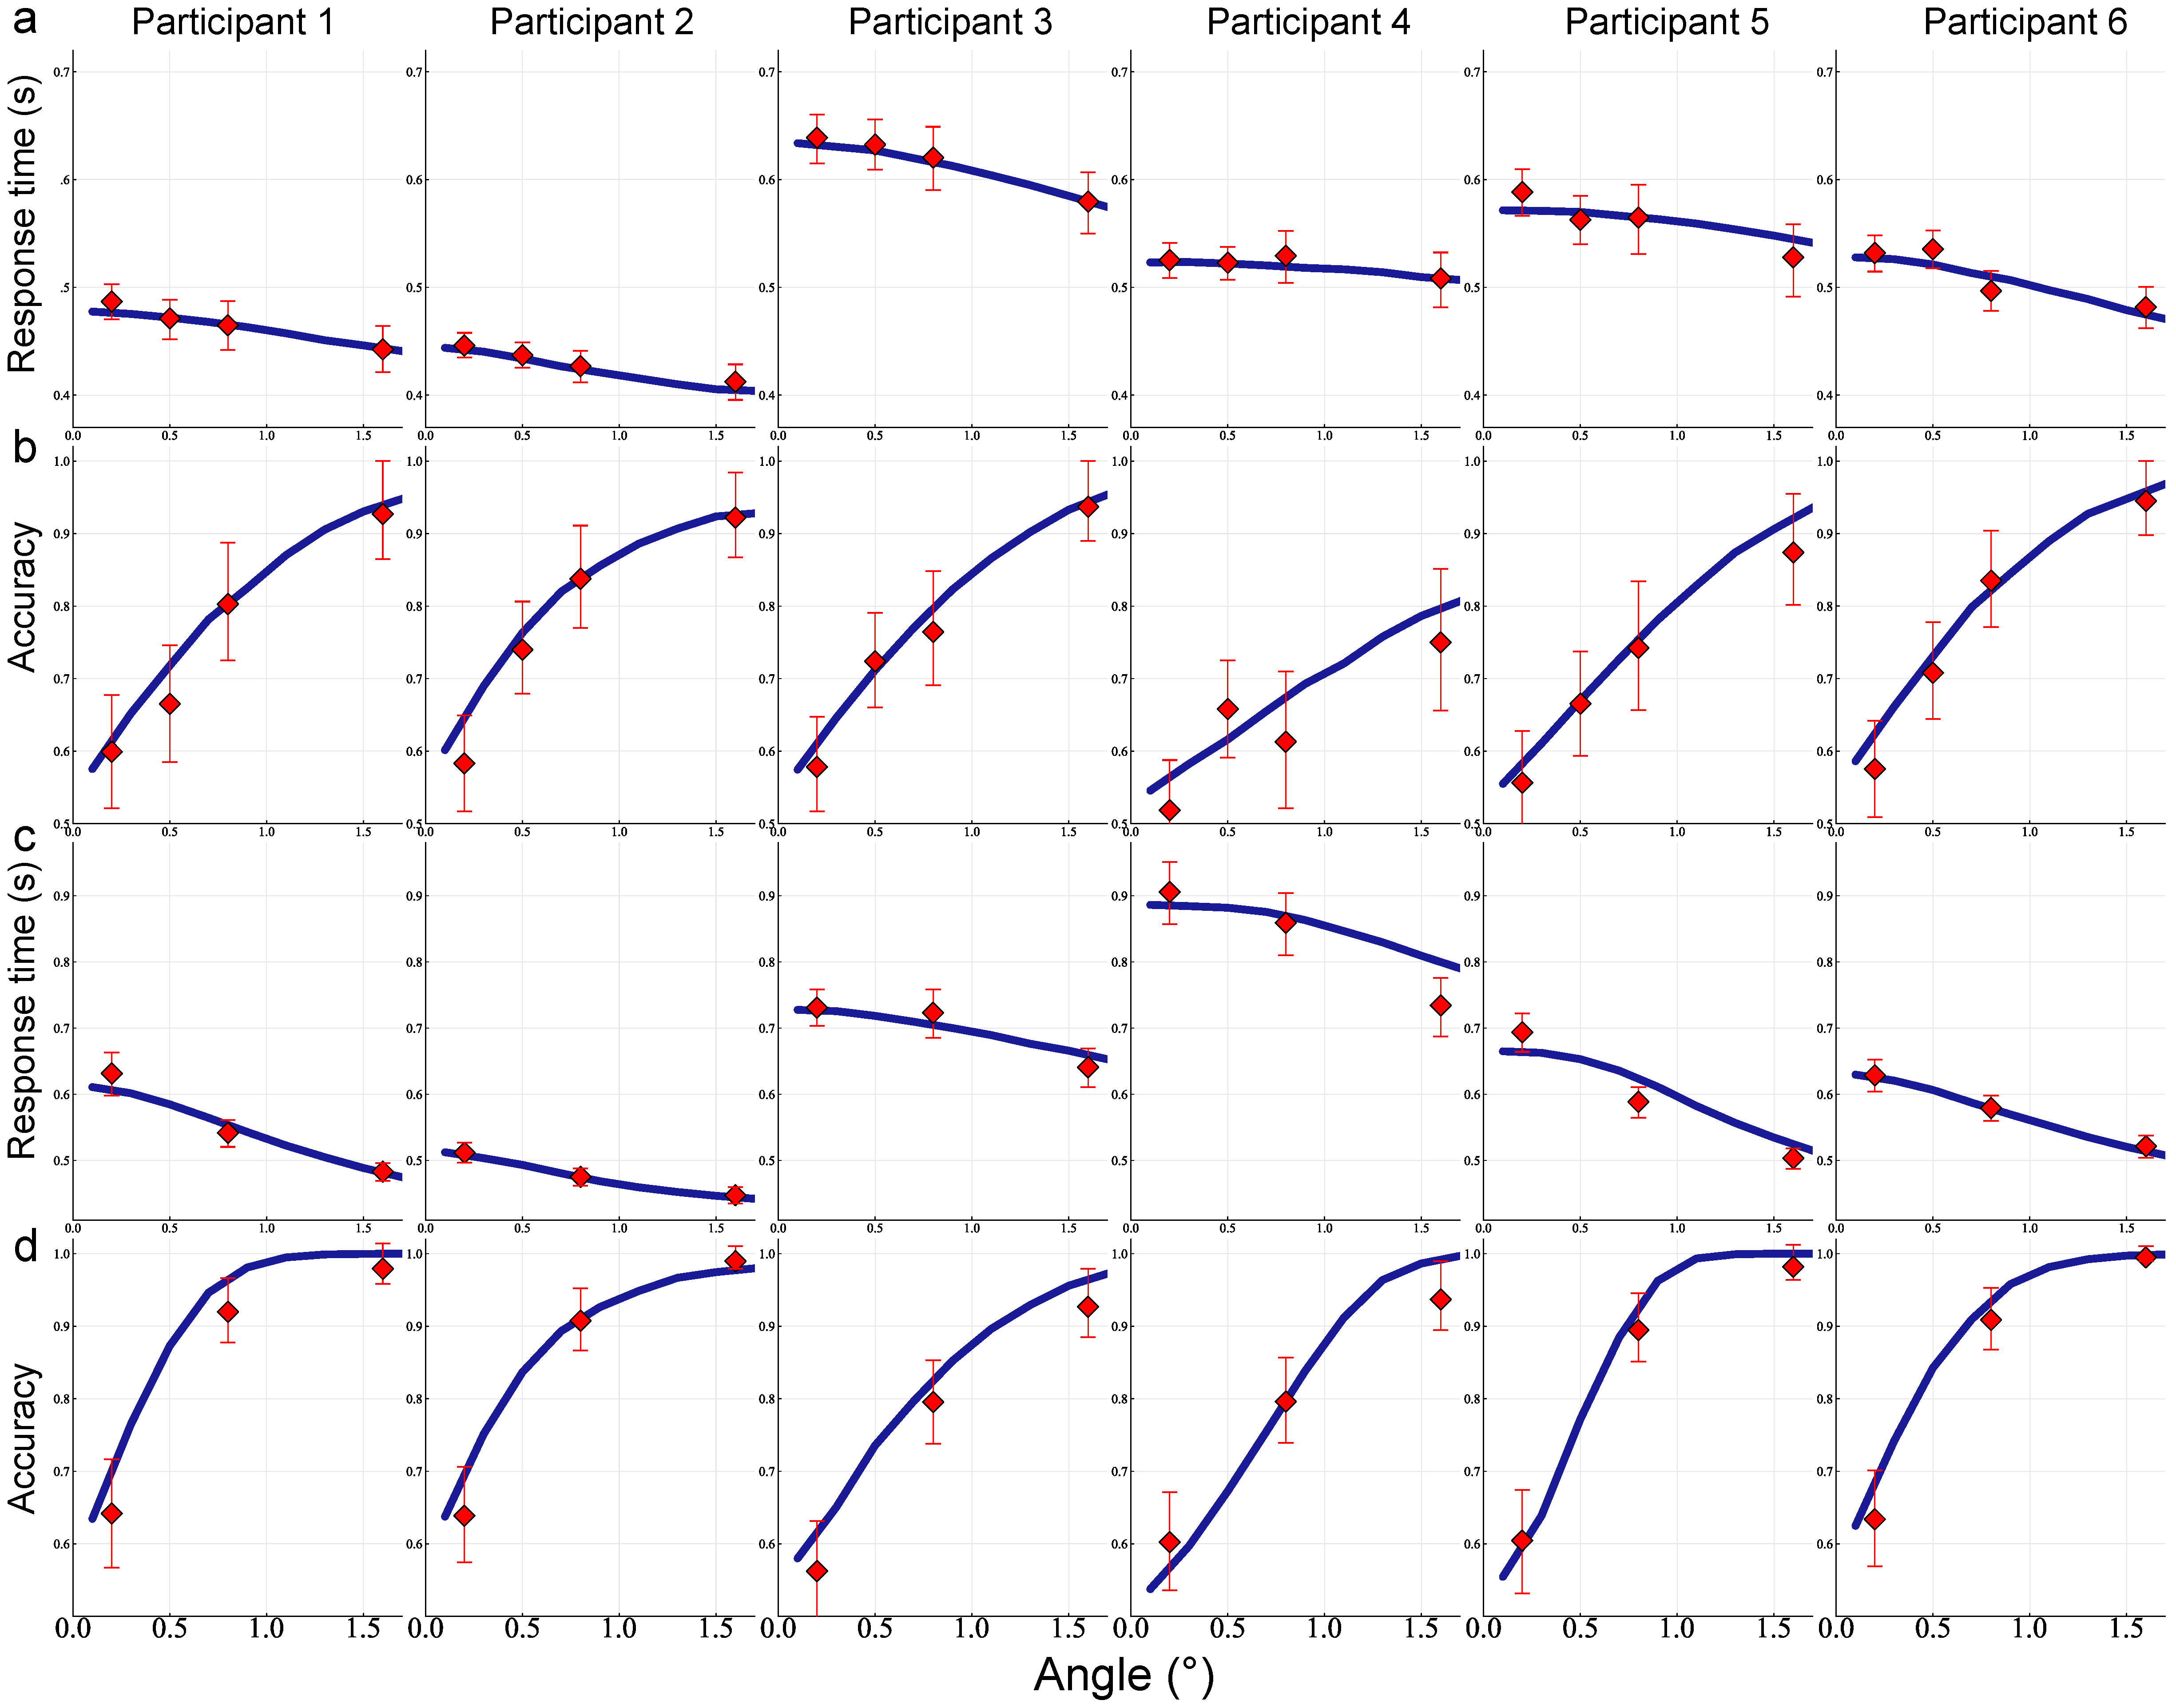
\includegraphics[width=1.0\linewidth]{Fig/Chapter4/fig3.eps}
%	\caption{{\bf Mean response times (A,C) and accuracies (B,D) as a function of the absolute value of stimulus orientation}, in the {\em pure} (A and B) and {\em confidence} (C and D) blocks. For each subject I represent the behavioral data (red dots) and the associated fitted model (blue line). Error bars are  $95\%$ confidence interval using the bootstrap method. }
%	\label{fig:chap4-fig3}
%\end{figure}

In Figure ???, I show the histogram
of the response times across participants for the pure and confidence blocks. The red curve shows the distribution
of non-decision times in the model, and the black curve the response times distribution of the model. One should note that, with a fit only based
on the mean response times and accuracies, the model also accurately account for the distributions of response times. I
find that the minimum value of non-decision time is $75$~ms for the pure block, and $100$~ms for the confidence block, and
the average non-decision times are within the order of magnitude of saccadic latency~\citep{luce1986response,Mazurek_A_2003}.
Finally, the NDT distributions clearly show a right skew for several participants, in
agreement with~\cite{verdonck2016factoring}. This justifies the modelling of non-decision times with an exponentially
modified Gaussian distribution (EMG), instead of simply adding a constant non-decision time to every decision time.
%%% phrase de conclusion ?
\begin{figure}[h!]
	\centering
	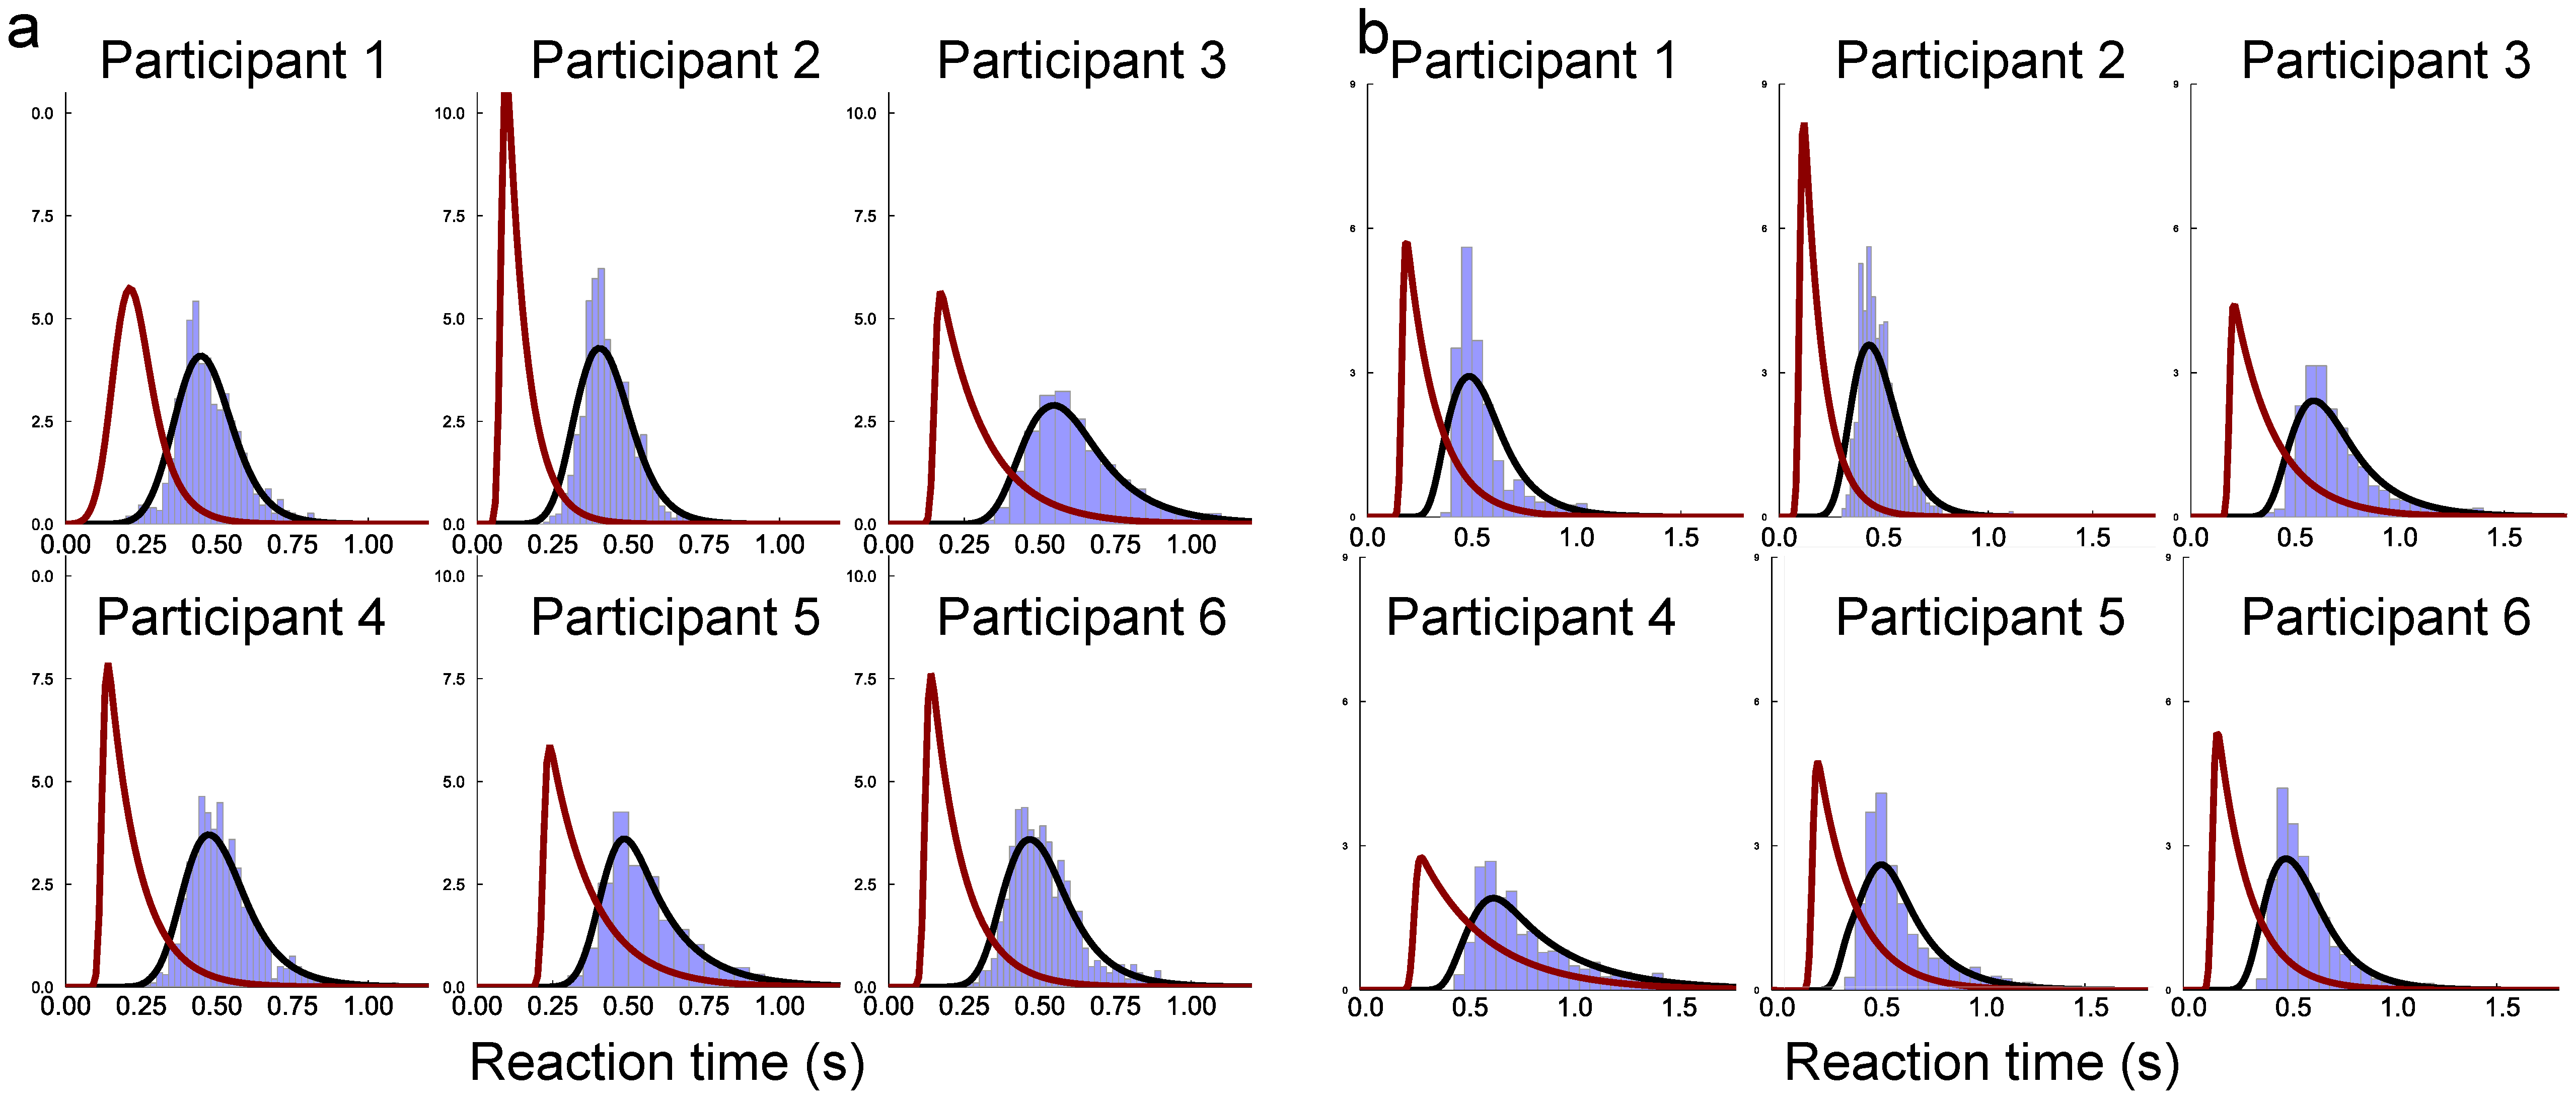
\includegraphics[width=1.0\linewidth]{Fig/Chapter4/fig4.eps}
	\caption{{\bf Distributions of RTs for each subject} (A) {\em Pure} block data, (B) {\em confidence block} data. For both panels:
	In blue, participants' histograms of the response times; Black curve: density of response times of the simulated network model; Red curve: the associated non decision response times distribution.}
	\label{fig:chap4-fig4}
\end{figure}





\subsection{Confidence model}
To model confidence within the attractor neural network, I made the hypothesis that the confidence in the decision is based on the difference $\Delta r$ between the neural activities of the winning and losing neural pools, measured at the time of the decision (balance of evidence) (see Figure ????). In the experiment of chapter ???, the measure of confidence is the one reported by the subjects on a discrete scale, and it is this reported confidence level that I want to model. I used the parameters obtained by the fitting procedure of the previous section (see Appendix ???), and the simulation protocol is similar to the experimental procedure. %% à détailler , où ça ?
Within this framework, I quantitatively link this empirical confidence to the neural difference $\Delta r$ by matching the distribution of the neural evidence balance with the empirical histogram of the confidence levels. This is done by using a procedure called {\emph histogram matching}~\citep{gonzalez2002digital} between the distribution of the neural balance of evidence and the discrete distribution of the reported confidence.

\begin{figure}[h!]
	\centering
	
\includegraphics[width=0.7\linewidth]{Fig/Chapter4/schemaConfiance.eps}
	\caption{{\bf Confidence matching procedure} TODO et à changer $z$ en $\theta$.}
	\label{fig:chap4-transfer-confidence}
\end{figure}


One important point of this analysis is that the shape of the mapping is not chosen a priori but non-parametrically inferred from the experimental data. This is in contrast with previous studies in which the sigmoidal shape is imposed~\citep{Beck_Probabilistic_2008,kepecs2008neural,Kepecs_A_2012,wei2015confidence}. However, I find that, for each participant, the mapping is well-approximated by a sigmoidal function of the type $1/\left(1 + \exp \left( - \beta \left( \Delta r - \kappa \right)\right) \right)$, with participants specific parameters $\kappa$ and $\beta$. %% TODO: ref Figure In~\cite{wei2015confidence}, the authors exhibit a link between a probabilistic measure of confidence and $\Delta r$, under
the form of a sigmoid function. The similarity of my findings thus suggests that the human reported confidence can be
understood as a discretization of a probabilistic function. 

\begin{figure}[h!]
	\centering
	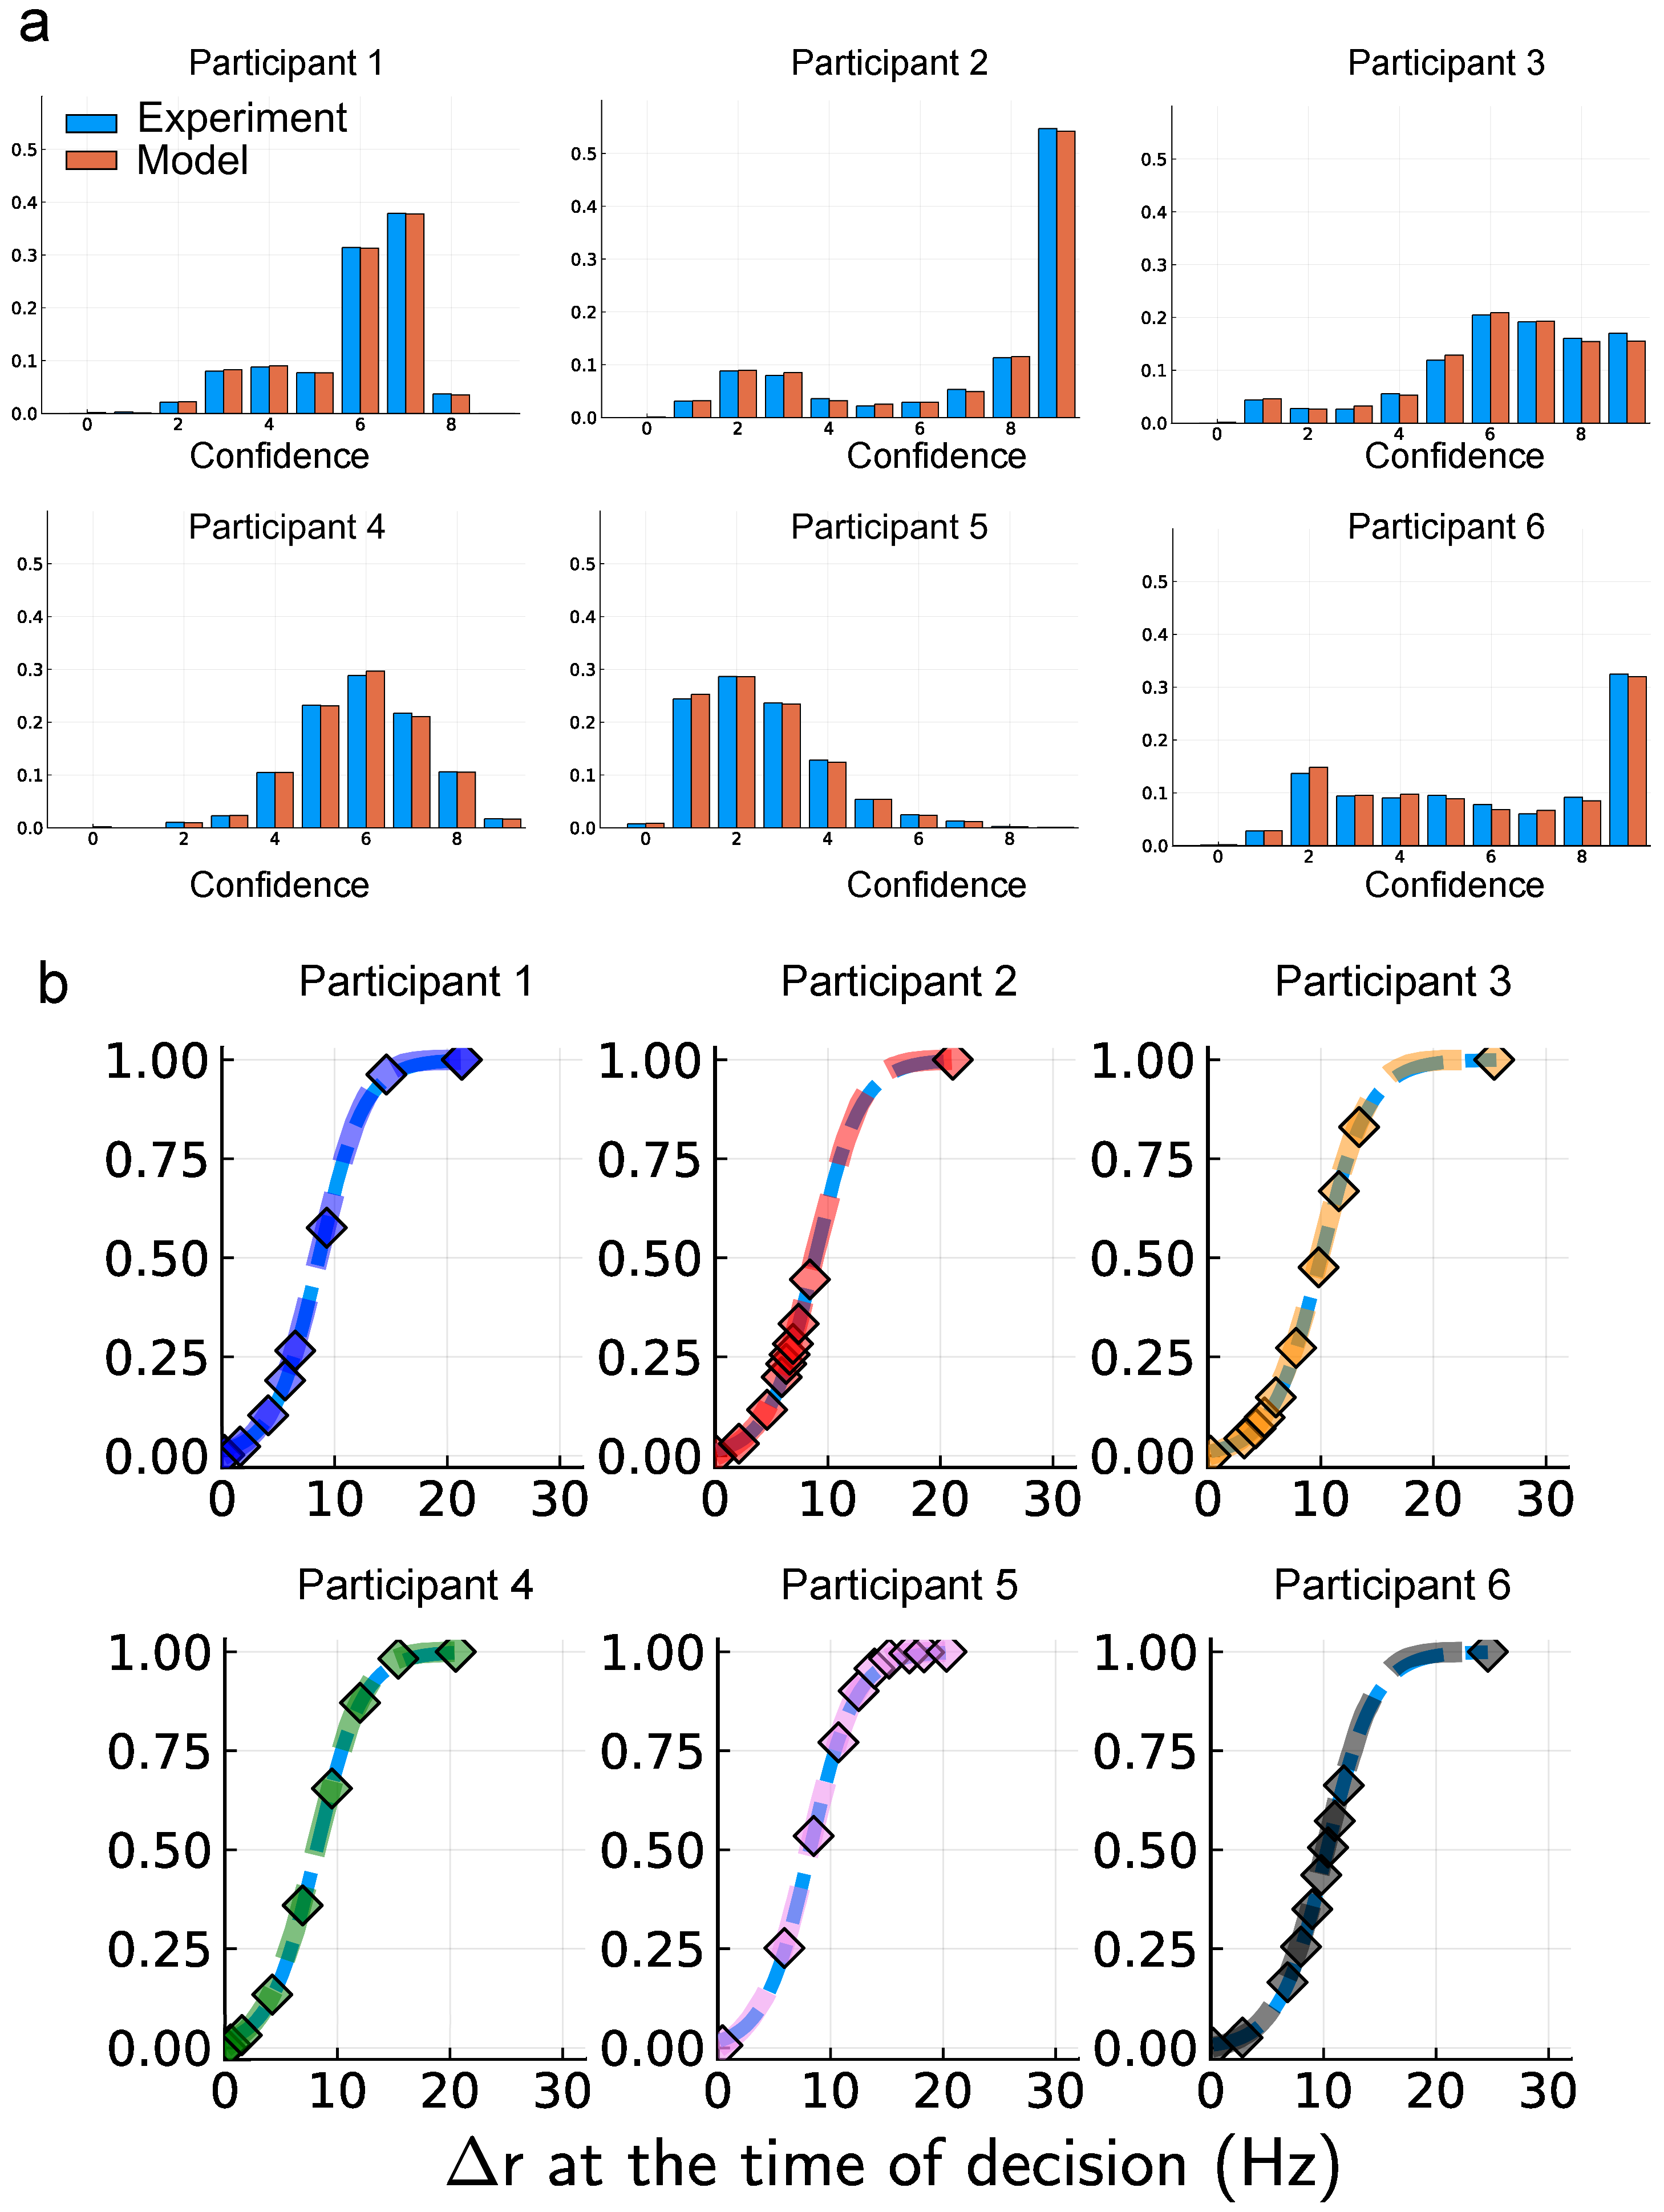
\includegraphics[width=0.7\linewidth]{Fig/Chapter4/fig5.eps}
	\caption{{\bf Matching network confidence measure to empirical behavioral confidence.}
	(A) Confidence histograms. The x-axis gives the value of the confidence on a discrete scale from 0 to 9.  Each sub-panel corresponds to a different participant with, in blue, the histogram of the reported confidence, and in orange, the one from the model. For clarity I plot the blue and orange bars side by side, but the bins of the histograms are, by construction, identical. (B) Transfer function $F$ for each participant. The x-axis denotes the difference in neural pools activities $\Delta r$ at the time of the decision, and the y-axis the cumulative distribution of $\Delta r$. Each point represents the levels of $\Delta r$ delimiting the level of confidence (from left to right, confidence level 0 to confidence level 9). The dashed colored curve is the cumulative distribution function (CDF) and the light blue dashed curve is the fit of the CDF by a sigmoid.}
	\label{fig:fig5}
\end{figure}


Studies have shown that confidence ratings are closely linked to response times~\citep{baranski1994calibration,desender2018post} and choice accuracy~\citep{peirce1884small,baranski1994calibration,sanders2016signatures,desender2018post}. Response time decrease and accuracy increases with confidence. In what follows, I study whether the neural balance of evidence can accounts for the link between the behavioral data: response times, accuracies and confidence reports. Figure ??? represents the response times (Figure ????) and choice accuracy (Figure???) with respect to the reported confidence level for each participant. The data points show the experimental results (with the error bars as the bootstrapped $95~\%$ confidence interval), and the colored line the result of the simulation (with the light colored area the bootstrapped $95~\%$ confidence interval).
I find a monotonic dependency between response times and confidence, and between accuracy and confidence, but with specific shapes for each participant. One should note that some values of confidence are only
observed for a few trials, resulting then in large error bars especially for accuracy as it consists in the mean of a binary variable. For the numerical simulations, the relatively large size of the confidence interval is due to the limited number of trials, since the simulation protocol is the same as the experimental one (same number of trials). These results show that an attractor neural network can correctly reproduces the psychometric and chronometric functions
with respect to confidence for each participant, despite the important difference of response times between participants.


\begin{figure}[h!]
	\centering
	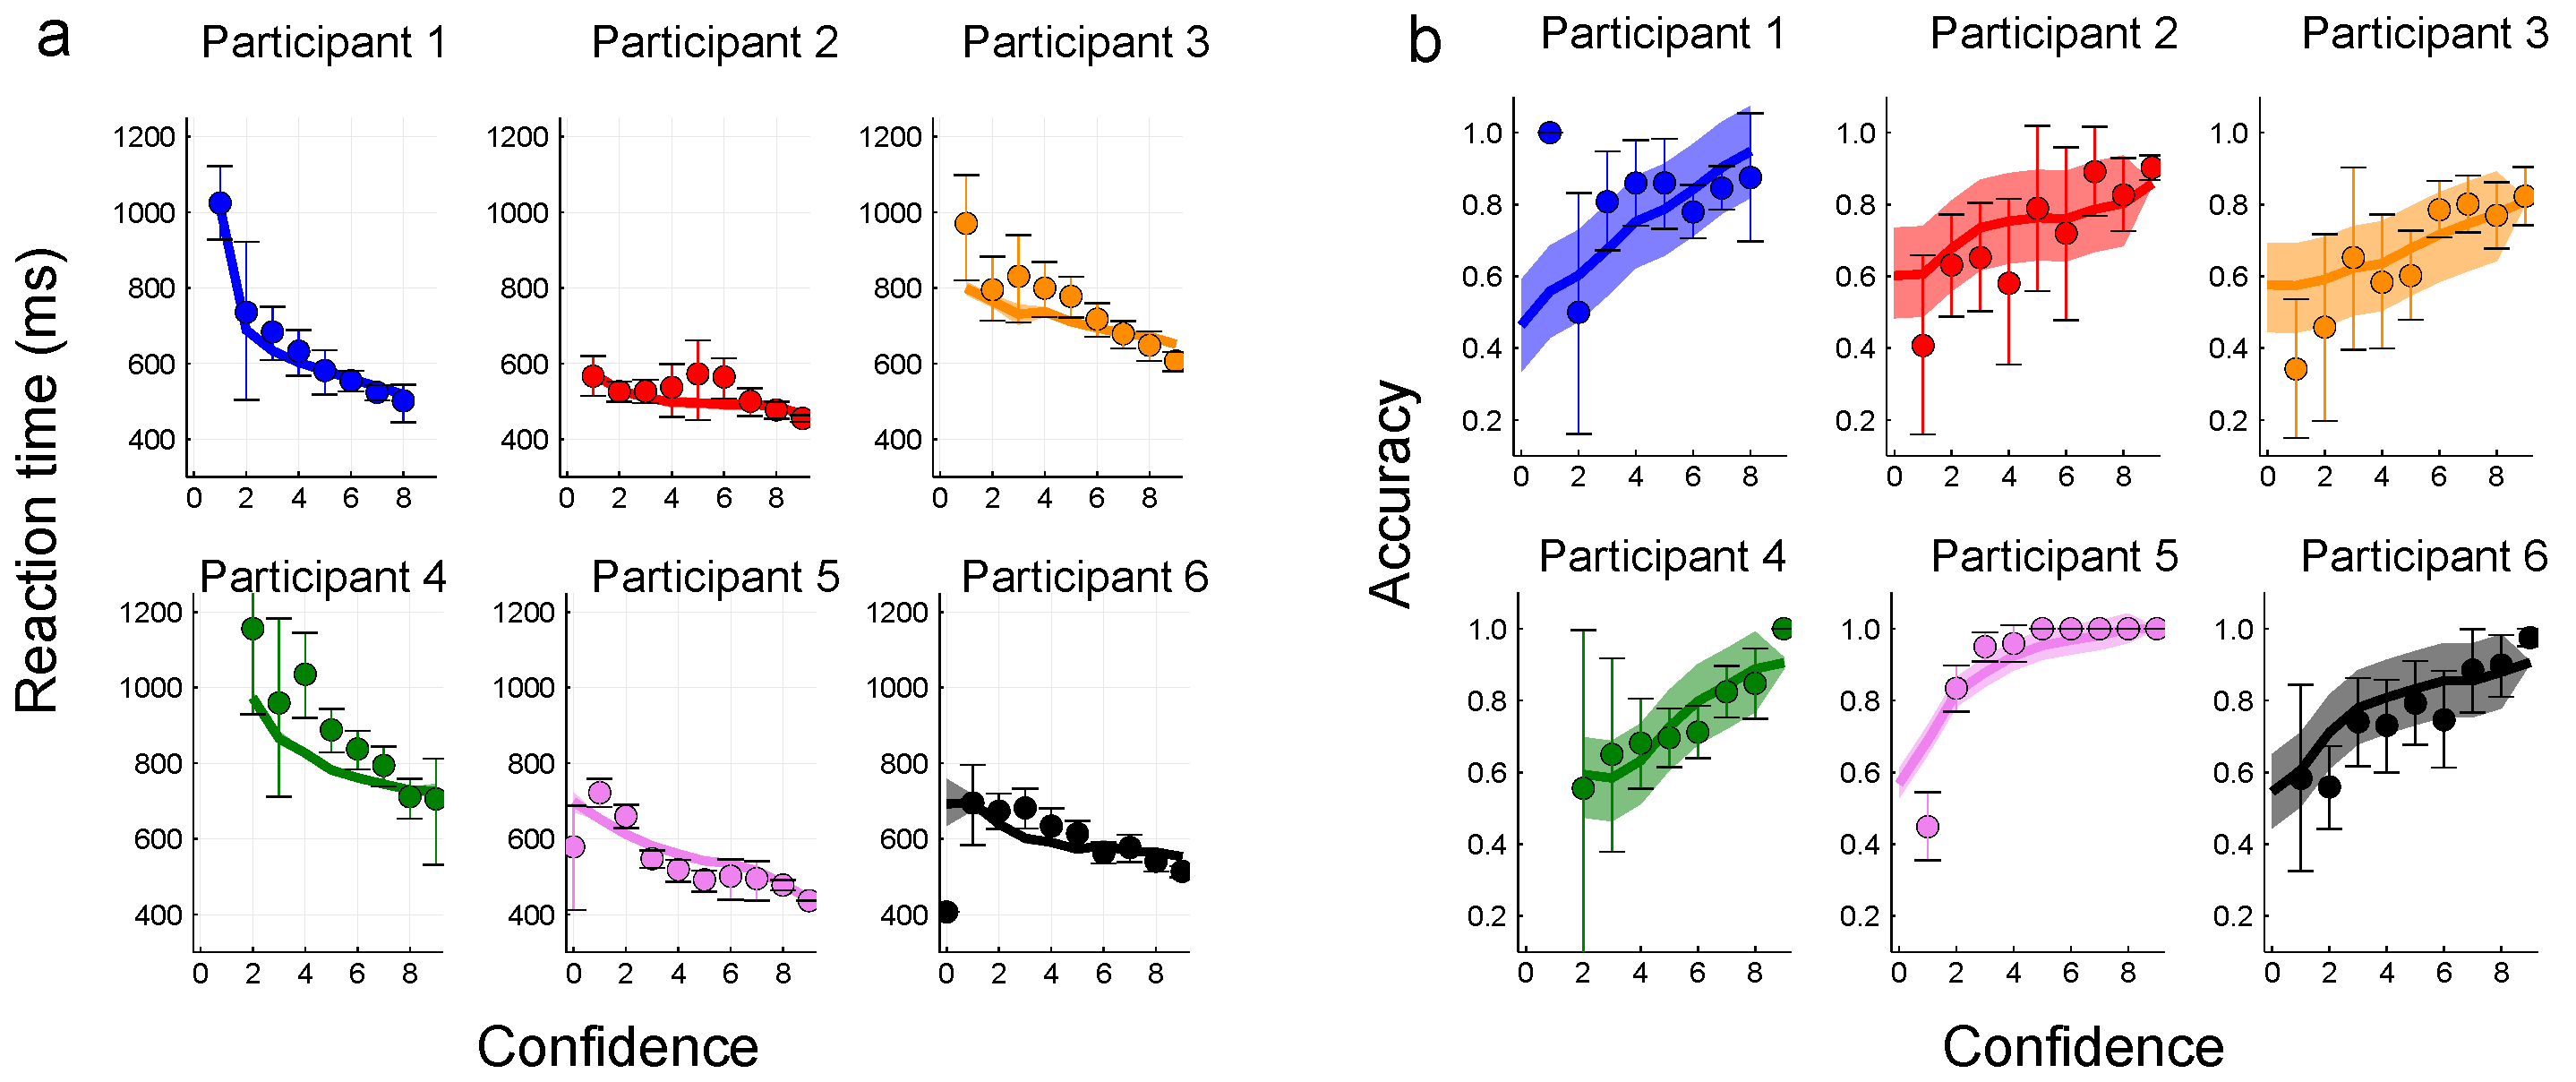
\includegraphics[width=1.0\linewidth]{Fig/Chapter4/fig6.eps}
	\caption{{\bf Response times and Accuracy as a function of confidence.}   (A) Response times, (B) Accuracy. For both panels: each sub-panel represents a different participant. Dots are experimental data with 95$\%$ bootstrapped confidence interval as error bars. Lines are averages over 20 simulations of the attractor neural network model. The shaded area represents the 95$\%$ bootstrapped confidence interval on the mean.
}
	\label{fig:fig6}
\end{figure}

%%% il va falloir rajouter des titres aux paragraphes
%% CONCORDANCE des TEMPS !!!!!!!!!!!!!!!!!!!!!!!!!!!!!!!!!!!!!!



\subsection{Sequential effects and confidence}

In chapter ???, I showed that an attractor neural network, using a simple relaxation dynamics, could reproduce various sequential effects observed in perceptual decision-making experiments such as history biases and post-error slowing. Very recently, the effects of confidence on the history biases have been experimentally investigated~\citep{braun2018adaptive,samaha2018confidence,desender2018a}. One main finding is that decisions with high confidence confer stronger biases upon the following trials. Here, I investigate the influence of confidence upon the next trial in the empirical data, and I will show that the results are well reproduced by the behavior of the dynamical neural model.


%% partie analyses à clarifier ?
First, I performed a statistical analysis of the effect of history biases on response times in the experimental data. To perform this analysis, I transformed the response times of each participant using the z-score~\citep{kreyszig1979advanced}. This allows us to study all participants together as the response times are now normalized.
I used RStudio~\citep{Rstudio} with the package {\it lme4}~\citep{lme4} to perform a linear mixed effects analysis~\cite{gelman2007data} of the history biases of the reaction times. The linear mixed effects model (LMM) I consider assumes that the logarithm of the response time at trial $n$, $RT_n$, is a linear combination of factors as follows:
\begin{equation}
\ln (RT_n) = a_{0,p} + a_{1,p} \vert \theta \vert + a_2 x_{\text{repetition}} + a_{3,p} \ln (RT_{n-1}) + a_4 \text{Conf}_{n-1}
\label{ModelLMM1}
\end{equation}
with $x_{\text{repetition}}$ a binary variable taking the value $1$ if the correct choice for the current trial is a repetition of the previous choice (and $0$ otherwise), $\theta$ the orientation of the Gabor (in degree), $RT_{n-1}$ the response times of the previous trials, and $\text{Conf}_{n-1}$ the confidence of the previous trial coded as $0$ for {\it low} and $1$ for {\it high}. The subscript $p$ in a coefficient (e.g $a_{0,p}$) indicates that  for this parameter is allowed a random slope per participant. For each participant, a trial is considered as low confidence (resp. high confidence) if the reported confidence is below (resp. above) the participant’s median

To ensure that the chosen model is the most preferable I compared it to other ones that do not include all the combination of factors. This comparison is done using the {\em ANOVA} function (with the lme4 package~\cite{lme4}) that performs model comparison based on the Akaike and Bayesian Information Criteria (AIC and BIC)~\citep{bates2014fitting}. Table~\ref{tableComparaison} presents the results of this comparison and shows that our LMM is preferable in all cases.

\begin{table}[!ht]
	\begin{flushright}
		\begin{tabular}{|l|l|l|l|l|l|l|}
			\hline
			{\bf } &  Df &  AIC   & BIC & LogLik. &  p value \\ 
			$a_{0,p} + a_{1,p} \vert \theta \vert + a_2 x_{\text{repetition}} + a_{3,p} \ln (RT_{n-1}) + a_4 \text{Conf}_{n-1}$ & 12 & -335 & -254 & 180 & \\
			$a_{0,p} + a_{1,p} \vert \theta \vert + a_2 x_{\text{repetition}} + a_{3,p} \ln (RT_{n-1}) $ & 11 & -324 & -249 & 173 & 0.0003 \\
			$a_{0,p} + a_{1,p} \vert \theta \vert + a_2 x_{\text{repetition}} $ & 7 & -4 & -42 & 9 & $<$2e-16 \\
			$a_0 + a_1 \vert \theta \vert + a_2 x_{\text{repetition}} + a_3 \ln (RT_{n-1}) + a_4 \ln (\text{Conf}_{n-1})$ & 7 & -225 & -177 & 119 & $<$2e-16\\
			$a_0 $ & 3 & -475 & -495 & -234 & $<$2e-16 \\
			\hline
		\end{tabular}
	\end{flushright}
	\caption{
		{\bf LMM tests on experimental data, models comparison. } The first row gives the tests for the LMM from Eq.~\ref{ModelLMM1}.  The p-values are for the tests based on BIC and AIC~\citep{bates2014fitting} between the LMM  from Eq.~\ref{ModelLMM1} and the one of the corresponding row.} 
	\label{tableComparaison}
\end{table}

%% mettre les coefficients dans la description ???

The results of the analysis of the experimental data are presented in Table~\ref{tableLMM1}. In line with previous work, higher orientations lead to faster response times and the repetition biases on response times~\citep{cho2002mechanisms}. Moreover, high confidence has the effect of speeding up the following trial. Finally, we find that the previous response time has an effect on the subsequent one, meaning that the participants have the tendency to show sequences of fast (or slow) response times.

\begin{table}[!ht]
	\centering
	\begin{tabular}{|l|l|l|l|l|ll|}
		\hline
		{\bf } &  Estimate &  Std. Error   & df & t-value & Pr &\\
		$a_{0,p}$  & $5.428$ & 1.466e-01 & $9.0$&  $37.038$ & $6.92\cdot 10^{-11}$ &*** \\
		$a_{1,p}$ & $-0.1027$ & $0.02390$  & $9.0$ & $-4.296$ & $0.002001$ &**  \\
		$a_2$ &  $-3.402\cdot 10^{-2}$ & $2.840\cdot 10^{-3}$  &$8.472\cdot 10^3$ &$-11.978$ & $< 2\cdot 10^{-16}$ &*** \\
		$a_{3,p}$ &  $1.517\cdot 10^{-1}$ & $1.651\cdot 10^{-2}$  & $7.0$ &  $9.187$ & $3.23\cdot 10^{-5}$ &***   \\
		$a_4$  & $-2.063\cdot 10^{-2}$ & $5.969\cdot 10^{-3}$ & $5.537 \cdot 10^3$  &$-3.456$ & $0.000553$ & ***\\
		\hline
	\end{tabular}
	\caption{
		{\bf Results of the application of the LMM from Eq.~\ref{ModelLMM1} on the experimental data.} $**$ stands for $p<0.005$ and $***$ for $p<0.001$.}
	\label{tableLMM1}
\end{table}

The next step is to investigate if the model can reproduce these various sequential effects, even being calibrated only on the mean response times, without the serial dependencies.  The results are shown in Table~\ref{tableLMMmodel} and I will summarize them below. The model captures the variation of response times with respect to angle orientation, as expected from~\cite{wong2006recurrent} and observed in the experiment. The repetition bias is correctly reproduced too. %% REFS ? 
Quite remarkably, the model shows an effect of confidence on response times, with a negative slope, as in the experiment.

\begin{table}[!ht]
	\centering
	\begin{tabular}{|l|l|l|l|l|ll|}
		\hline
		{\bf } &  Estimate &  Std. Error   & df & t value& Pr & \\
		$a_{0,p}$  & $5.999$  &  $0.08032$ & $4.229$  & $74.690$ & $9.22\cdot 10^{-8}$& ***  \\
		$a_{1,p}$ & $-0.01744$ & $5.551\cdot 10^{-4}$ & $2.886$ &$-31.420$&  $9.47\cdot 10^{-5}$ &*** \\
		$a_2$ &$-0.1814$&  $8.133\cdot 10^{-3}$ & $4.822 \cdot 10^3$  &$-22.301$ & $< 2\cdot 10^{-16}$ &*** \\
		$a_{3,p}$ &  $-0.02075$ &$1.545\cdot 10^{-2}$& $4.628$ & $-1.343$&  $0.24139$  &   \\
		$a_4$ & $-0.02324$  &$8.336\cdot 10^{-3}$ &  $4.847\cdot 10^3$  &$-2.788$  & $0.00533$ &**\\
		\hline
	\end{tabular}
	\caption{
		{\bf Results of the application of the LMM from Eq.~\ref{ModelLMM1} on the data from the neural network simulations.} $**$ stands for $p<0.005$ and $***$ for $p<0.001$.}
	\label{tableLMMmodel}
\end{table}

%% Paragrpahe repris assez fortement de l'article (celui du dessus également
\paragraph*{Underlying neural dynamics.} The analysis of the dynamics performed to understand how the neural dynamics leads to these confidence-specific effects is similar to the one done in chapter ???. %% REFS ?
Figure ??? presents the result of this analysis. 
On each panel, I compare
the mean neural dynamics for post-low and post-high confidence trials (respectively red and blue lines). Without loss of
generality, one can assume that the previous decision was a C grating (clockwise). The relaxation dynamics between
two consecutive trials are different, resulting in different starting points for the next trial, from post-low and post-high confidence trials. Panel (A) corresponds to the case where the new stimulus is also C oriented ("repeated" case), at low strength level. The ending points of the relaxations fall into the correct basin of attraction. Because the post-high confidence relaxation lies deeper into the basin of attraction than the one of post-low trials, the subsequent dynamics will be faster for post-high confidence trials in this case. Panel (B) represents the case, still at low stimulus strength, where the stimulus orientation of the new stimulus is the opposite ("alternated" case) to the one corresponding to the previous decision (hence an AC grating). Both dynamics lie close to the basin boundary of the two attractors, thus the dynamics are slow and there is no significant difference between post-low and post-high confidence trials. In panels (C) and (D) we represent the same situations as panels (A) and (B), respectively, but for high strength levels (easy trials). The ending points of the relaxations are far from the boundary of the basins of attraction, whatever the grating presented. The response times for post-high and post-low confidence trials are thus similar. This analysis shows that the non-linearity of the network dynamics is responsible for the considered sequential effect. Indeed, in the absence of non-linearity, the repeated and alternated case would compensate each other and there would be no specific effect related to the basin boundaries.
%%% discuter l'analyse plus en détail qui a été faite

The next step is to step this analysis of the dynamics of the model with the experimental data. To do so, I regrouped the response times of the experiment into the same categories: high and low stimulus strength, repeated or alterned trials. Within each of these four categories, I compare the post-high and low confidence trials, using a t-test~\citep{fay2010wilcoxon}. The results are the following: mean response times between post-low and high confidence trials are different in the low orientation and repeated case (t-test, $p=0.044$), but are identical in the three other cases. %% plus de détails ?
%%% attention erreur dans l'article à corriger.
This is an important point, as the dynamics of the model does not only reproduce the global effect of confidence on the next trial, but also difference between high and low orientations trials. 

%%% détail sur la répétition des temps de réponse ???




\subsection{Attractor neural networks vs. other models} %% titre à change surement (sauf si on en fait une conclusion de partie carrément ---> à réfléchir de si on compara avec les DDM !!!

As discussed previously, various models have been proposed in order to model confidence during decision-making. Here, I will compare our model with other models that have been proposed. Previous studies found that, during a perceptual task, reported confidence increases with stimulus strength for correct trials, but decreases for incorrect trials~\citep{kepecs2008neural,sanders2016signatures,desender2018a}. %% commentaire de plus ?
This effect is in accordance with a prediction of statistical confidence, defined as the Bayesian posterior probability that the decision-maker is correct~\citep{griffin1992weighing,sanders2016signatures}. I investigated this effect with our framework. Figure ??? represents the mean confidence as a function of stimulus strength, for correct and error trials. One can note that, indeed, the participants exhibit this behavior but that the attractor neural network is able to capture this tendency. Thus, an attractor network model of decision-making reproduces a key feature of statistical confidence.

Another question one could ask is how does the attractor network model performs with respect to other dynamical models ? To address this question I will consider another non-linear model that has been used to model decision-making, the Usher-McClelland model~\citep{usher2001time}. The equations of this model are the following:
%% diff commande
%% vérifier si besoin de mettre les équations suivant l'introduction qui sera faite
\begin{align}
    \tau d x_1 &= - k x_1 dt - \beta  f(x_2) dt + I_1 + \sigma \mu_1 (t) \\
    \tau d x_2 & = - k x_2 dt - \beta f(x_1) dt + I_2 + \sigma \mu_2 (t)
\end{align}
with $\mu_i(t)$ a white noise process and $I_i$ the input current to the system. The external input is defined as $I_i = 0.5 \pm c_{\theta}$, with $c_{\theta}$ the strength per angle as in the attractor neural network. $\sigma =0.4$ denotes the strength of the noise, $k$ the relaxation strength, $\tau=0.1$ the relaxation time and $\beta$ the inhibitory term. Finally, the function $f$ is a sigmoidal function of gain $G=0.4$ and half-activity offset $d=0.5$, $f(x_i) = 1/ \left[1 + exp \left( -G(x_i -d\right) \right]$. The dynamics occurs until a threshold $z$ is reached for one of the two units. It should be noted that, despite the non-linearity, the Usher-McClelland model is closer to drift-diffusion models than to biophysical attractor model. This is principally due to the fact that the only non-linearity is in the interaction between both units. Thus, reductions to one-dimensional drift diffusion models can be made in various ranges of parameters~\citep{bogacz2006physics}.

I fit this model to the experimental data using the same procedure as for the attractor neural network (see Appendix ?? for more details). The resulting parameters are the following:
%% à insérer

The next step is to define confidence in a similar way as with the attractor model using the balance of evidence and the histogram matching procedure.
%% courbes des performances ?
Figure ?? presents the relation between reaction times, accuracies and confidence for this model. At first sight the fit between numerical simulations and experimental data looks accurate. However, it is only true for intermediate value of confidence. For some of the participants (Participant 1, 4 and 5), there is a strong divergence of the model at high confidence. This can be understood by the fact that, in this model, {\em firing rate} variables can take negative values (the steady state corresponds to a symmetric state with negative values). This leads to extreme values of confidence for long trials. Moreover, for some participants (such as 1 and 4), the trend in accuracy, despite being always increasing, is not correct. This highlights the fact that, even with the same model for confidence, discrepancies between models of decision-making exist. It is then possible to distinguish different models by comparing them on different aspect of decision-making. %% ccl à changer ? 

Finally, the last model I will compare to the attractor model is the independent race model (IRM). I chose this model because it is possible to define confidence using the balance of evidence. Such models have been successfully used to model decision-making experiments. %% REFs et refs des équations
I will investigate the notion of sequential effects with the IRM. As already mentioned in a previous chapter, when studying sequential effects with models such as the IRM, the parameters are allowed to change between each condition. This characteristic does not seem to be biophysically plausible %% à détailler ??
and, to compare with the attractor network, it is necessary to extend the IRM with a relaxation dynamics. After a decision is made, both units receive a non-specific inhibitory input leading to a relaxation until the next stimulus is presented (Figure ??). Within this extended IRM framework, one can study how the sequential effects would be correlated with confidence in an IRM model with a fixed set of parameters.


% 
Since in the IRM there is no interaction between the two races, the relaxation of the winning race is the same in both low and high confidence trials. However, the ending point of the relaxation following a decision is closer to the base-line (0 line) for a high confidence trial than when it comes to a trial with low confidence trial (Figure ???). For the next trial, if the winning race is the same as previously, then the mean response times are identical in low and high confidence cases. However, if the opposite decision is made, the response time in the post-low confidence case is faster than the one in the post-high confidence case (Figure ???).%%% TODO
This behavior is in contradiction with the experimental data for which the opposite effect is observed.
This conclusion applies more generally to any race-type model without interactions between units.
%% ou mettre les paramètres du fit ?

%ù Question JP: le chapitre est-il cohérent où trop proche de l'article ?

%% check concordance des notations mathématiques
%%%% 
%% Discussion del 'article de Wei Ji ma en fin de chapitre ou en conclusion finale ??
%%

%% Plus de conclusions ????
\end{comment}